\subsection{Analysis strategy}

\begin{frame}{Object and event selection}

\begin{columns}
\column{0.6\textwidth}

\begin{itemize}
    \item \textbf{Di-photon trigger} (83\% efficiency for signal)
    \item Neural Network primary vertex
    \item \textbf{$\geq $ 2 Tight} and \textbf{isolated} \textbf{photons} (\textbf{\textcolor{HHturquoise_d}{H$\to\gamma\gamma$}}):
    \begin{itemize}
        \item $\frac{p_{T}^{\gamma}}{m_{\gamma\gamma}} > $ 35\% (25\%) for leading (subleading)
    \end{itemize}
    \item \textbf{Exactly 2 $b$-jet} (\textbf{\textcolor{HHred}{H$\to b\bar{b}$}}):
    \begin{itemize}
        \item particle flow jet ($p_{T} > $ 25 GeV \& $|\eta| < $ 2.5)
        \item $b$-tagging: DL1r with 77\% efficiency
    \end{itemize}
\end{itemize}



\textcolor{gray}{less than 6 jets} \\
\textcolor{gray}{zero leptons (electrons or muons)}

\column{0.4\textwidth}

\begin{figure}
    \centering
    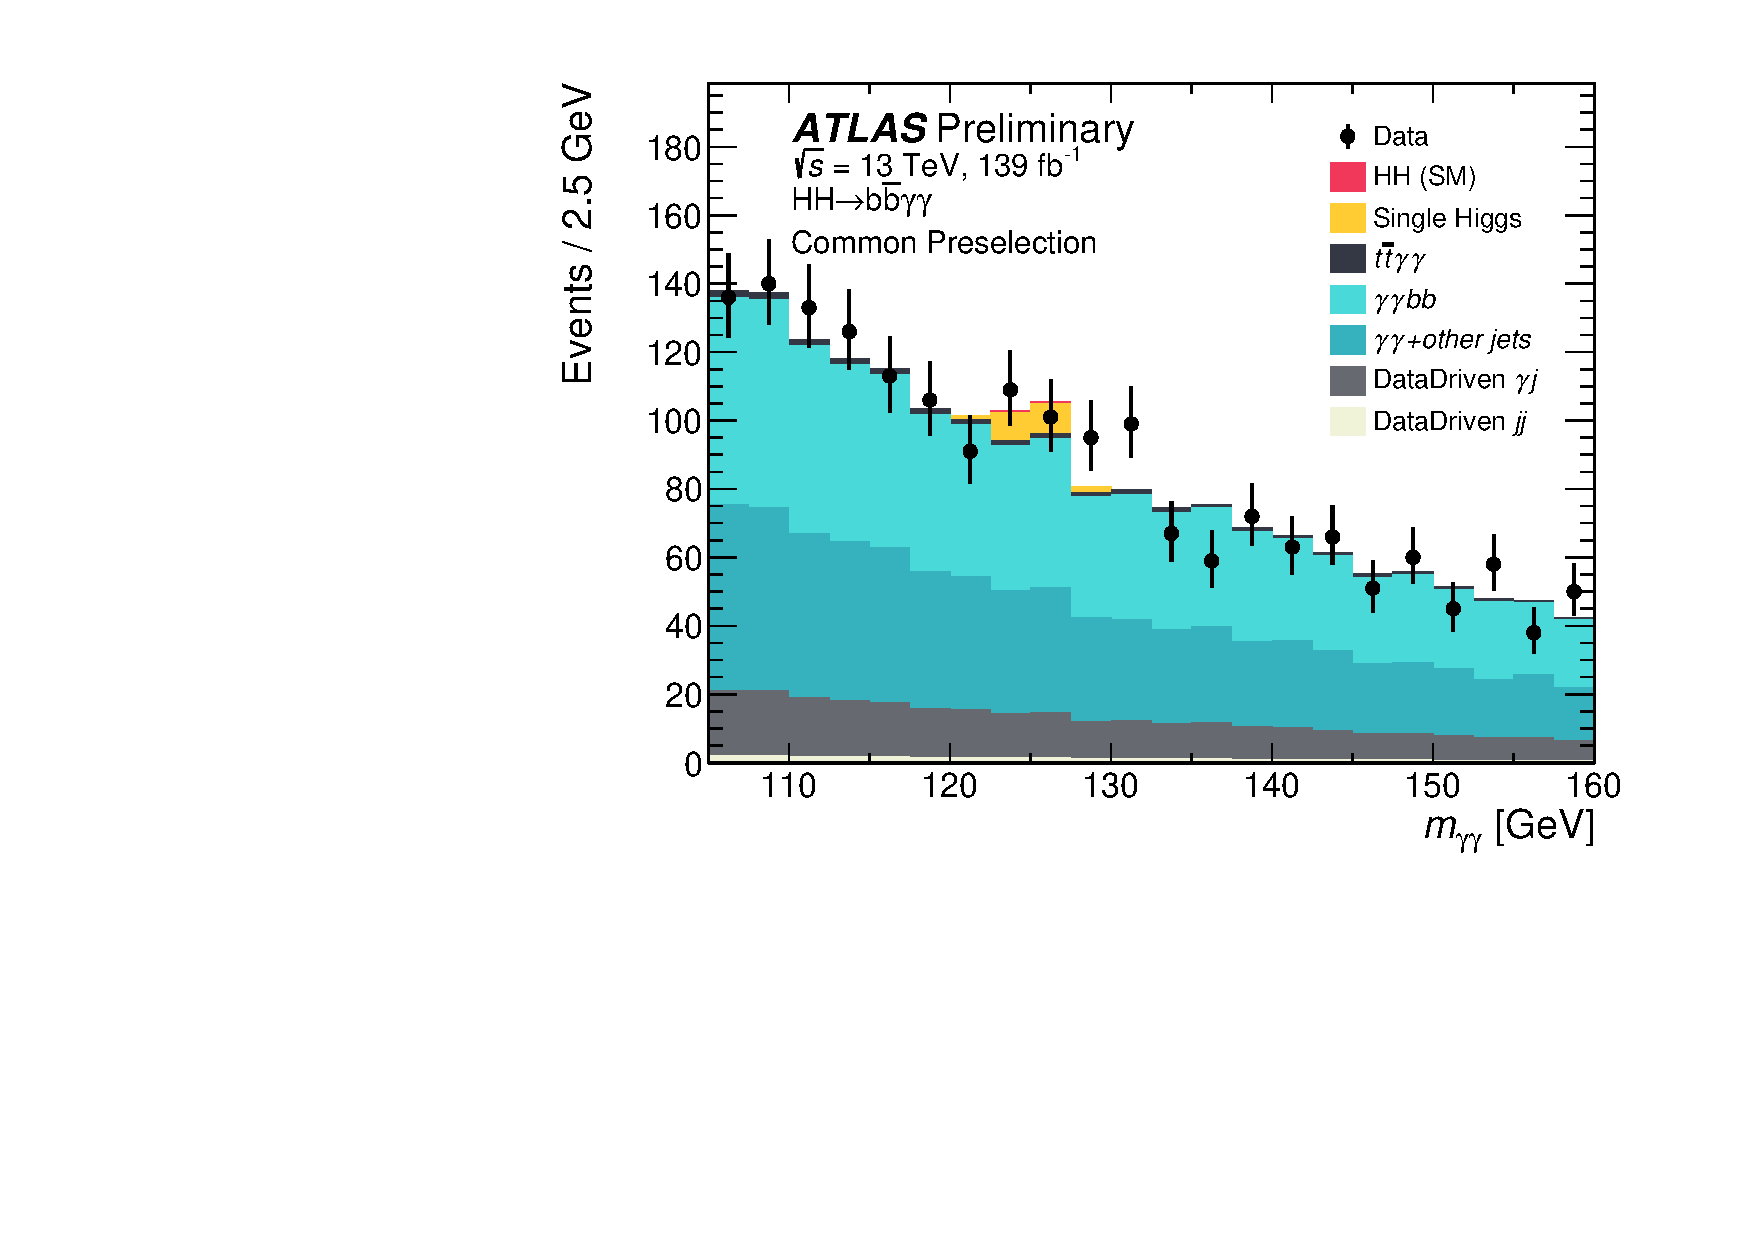
\includegraphics[width=1.1\textwidth]{Part3/Img/myy_common.pdf}
    
\end{figure}

%\begin{figure}
%    \centering
%    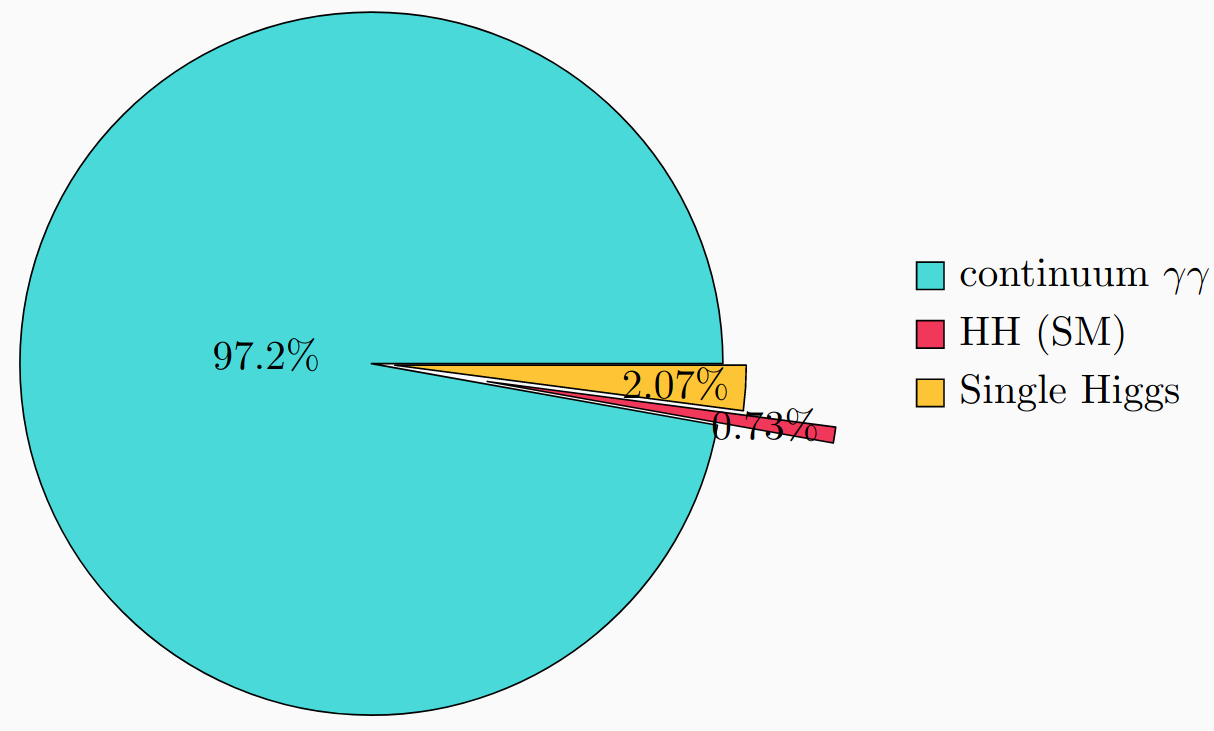
\includegraphics[width=0.7\textwidth]{Part3/Img/pie.png}
%\end{figure}

\end{columns}

\end{frame}

\begin{frame}{$b$-jet energy calibration}
\begin{columns}
\column{0.4\textwidth}
\begin{figure}
    \centering
    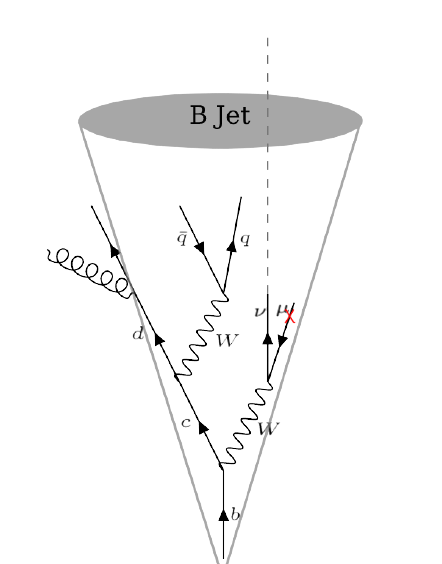
\includegraphics[width=0.8\textwidth]{Part3/Img/b-jet-nobkg.png}
\end{figure}

\column{0.6\textwidth}

\begin{itemize}
    \item $m_{b\bar{b}}$ highly discriminating for H$\to b\bar{b}$
    \item $\sigma_{m_{b\bar{b}}}\sim$ 16 GeV, $\sigma_{m_{\gamma\gamma}}\sim$ 2 GeV
    \item Standard calibration not enough, due to: 
    \begin{itemize}
        \item \textcolor{HHred}{\textbf{semi-leptonic}} decay $\to$ \textcolor{HHturquoise_d}{\textbf{missing neutrino}}
        \item \textcolor{HHturquoise_d}{\textbf{large $b$-quark mass}}
    \end{itemize}
\pause    
    \item Decoupled $b$-jet energy calibration method
    \begin{itemize}
        \item Adding soft muon, \textcolor{HHred}{\textbf{$\mu$-in-jet correction}}
        \item $p_T$ rescaling, \textcolor{HHturquoise_d}{\textbf{$p_T$Reco correction}}
    \end{itemize}
\end{itemize}
\end{columns}
\end{frame}

\begin{frame}{$b$-jet energy calibration}
\begin{columns}
\column{0.5\textwidth}
\begin{itemize}
    \item \textcolor{HHred}{\textbf{$\mu$-in-jet}}
    \begin{itemize}
        \item Adding back \textbf{medium} muons
        \item Variable $\Delta R$ 
    \end{itemize}
    \item \textcolor{HHturquoise_d}{\textbf{$p_T$Reco}}
    \begin{itemize}
        \item $p_T$-dependent scale factor
        \item Computed on \textbf{$t\bar{t}$ sample}
    \end{itemize}
\end{itemize}
\begin{figure}
    \centering
    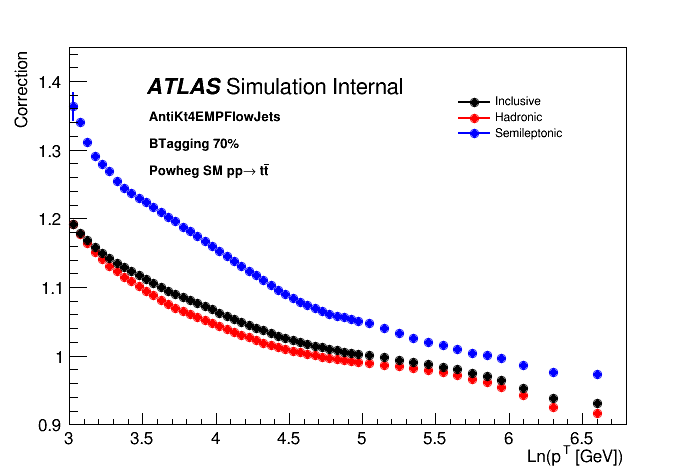
\includegraphics[width=0.8\textwidth]{Part3/Img/ptrecopflow.png}
\end{figure}

\column{0.5\textwidth}
\begin{itemize}
    \item Applied to HH$\to b\bar{b}\gamma\gamma$ $b$-jets
\end{itemize}
\pause
\visible<2>{
\begin{figure}
    \centering
    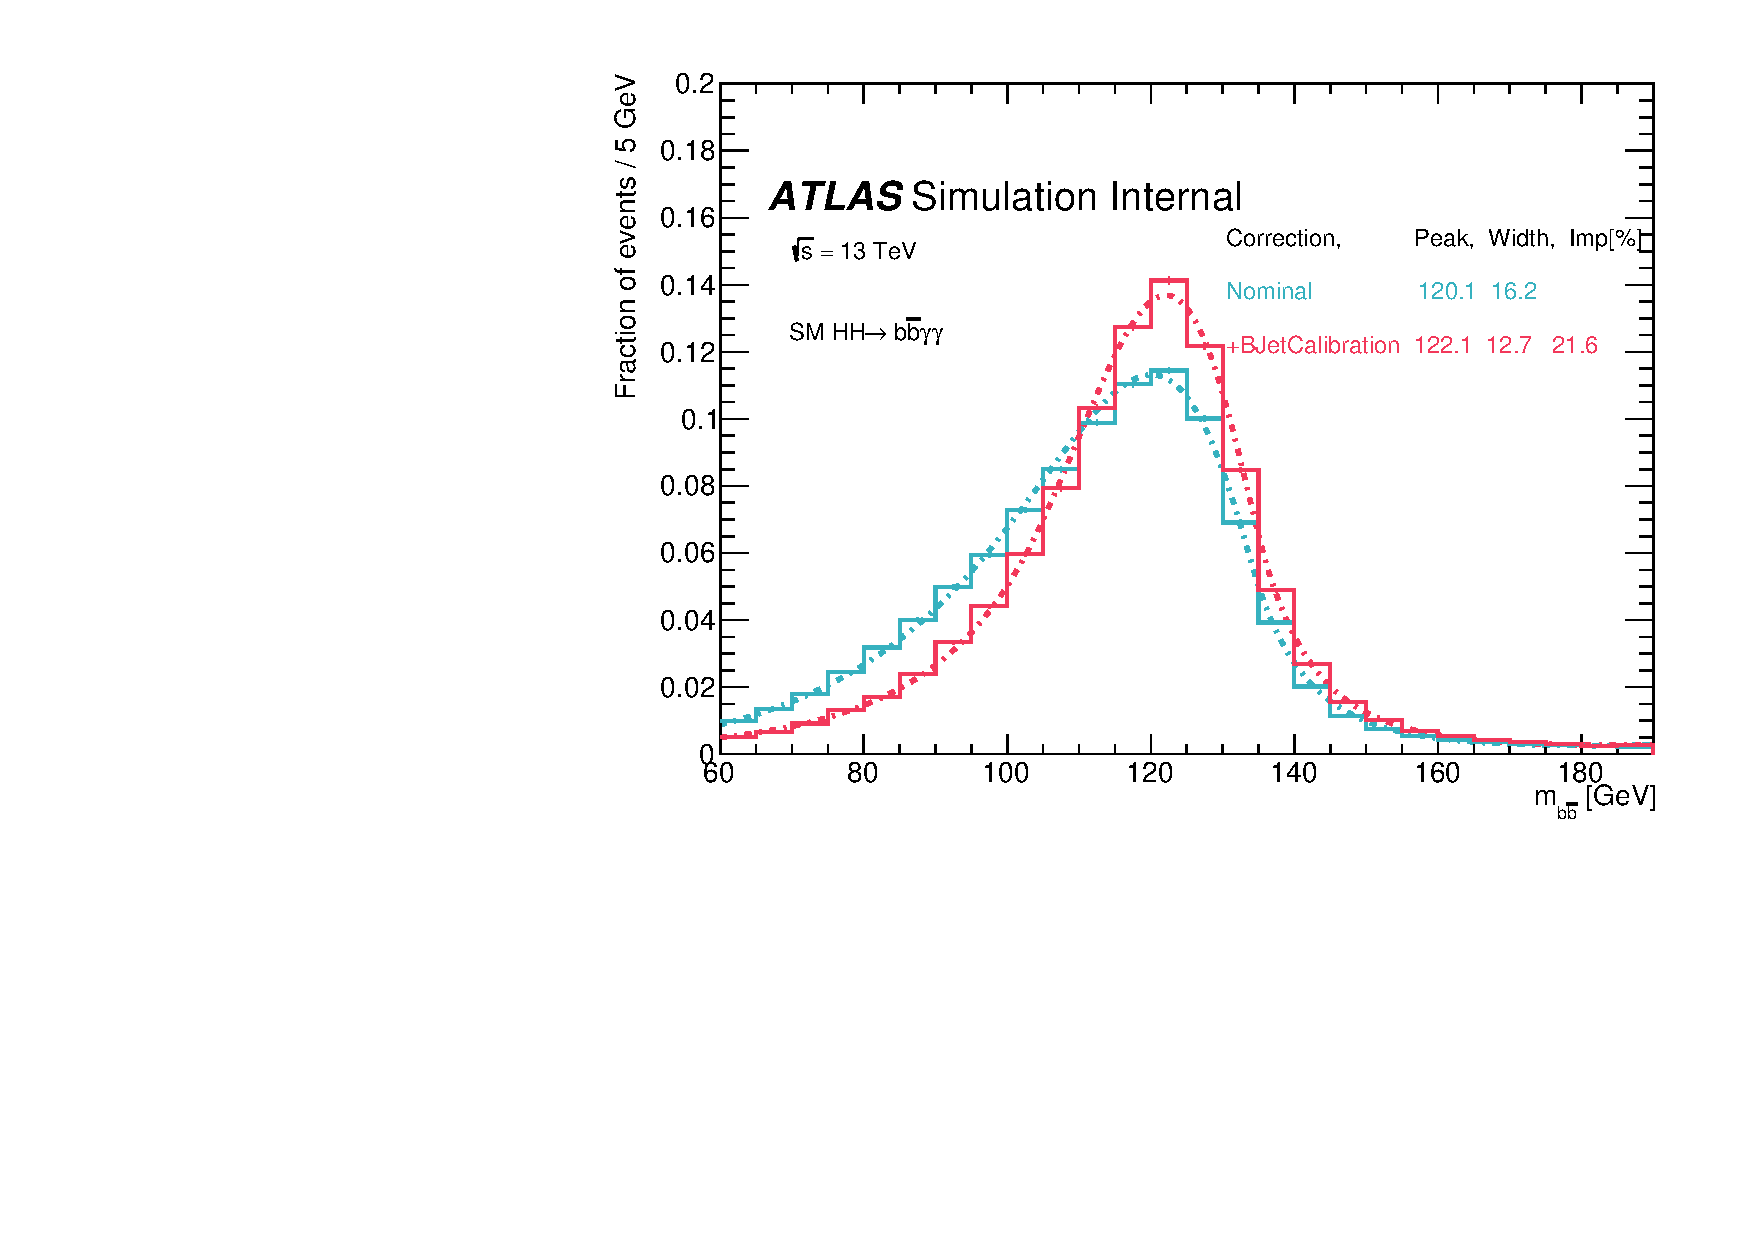
\includegraphics[width=0.9\textwidth]{Part3/Img/mbb_Paper.pdf}
\end{figure}
}
\begin{itemize}
    \item \textcolor{HHred}{\textbf{$\sim$ 22\%}} imp. on $m_{b \bar{b}}$ resolution
    \item \textcolor{HHred}{\textbf{7\%$\pm$2\%}} imp. on expected significance
\end{itemize}

\end{columns}    
\end{frame}


\begin{frame}{Categorization strategy}

\begin{columns}
\column{0.5\textwidth}
\begin{itemize}
    \item Sensitivity to:
    \begin{itemize}
        \item \textbf{\textcolor{HHred}{SM HH signal}}
        \item \textbf{\textcolor{HHturquoise_d}{
BSM scenarios}}
    \end{itemize}
\pause    
    \item Two regions on $m_{b \bar{b}\gamma\gamma}^{*}$
    \begin{itemize}
        \item \textbf{High mass $m_{b \bar{b}\gamma\gamma}^{*} >$ 350 GeV}, \textcolor{HHred}{$\sigma_{HH}$ limit}
        \item \textbf{Low mass $m_{b \bar{b}\gamma\gamma}^{*} <$ 350 GeV}, \textcolor{HHturquoise_d}{$\kappa_{\lambda}$ variations}
    \end{itemize}
\end{itemize}

\begin{itemize}
    \item Signal-background separation: \textbf{MVA}
\end{itemize}

\column{0.5\textwidth}

\begin{figure}
    \begin{overprint}
    \onslide<1>\centering\centering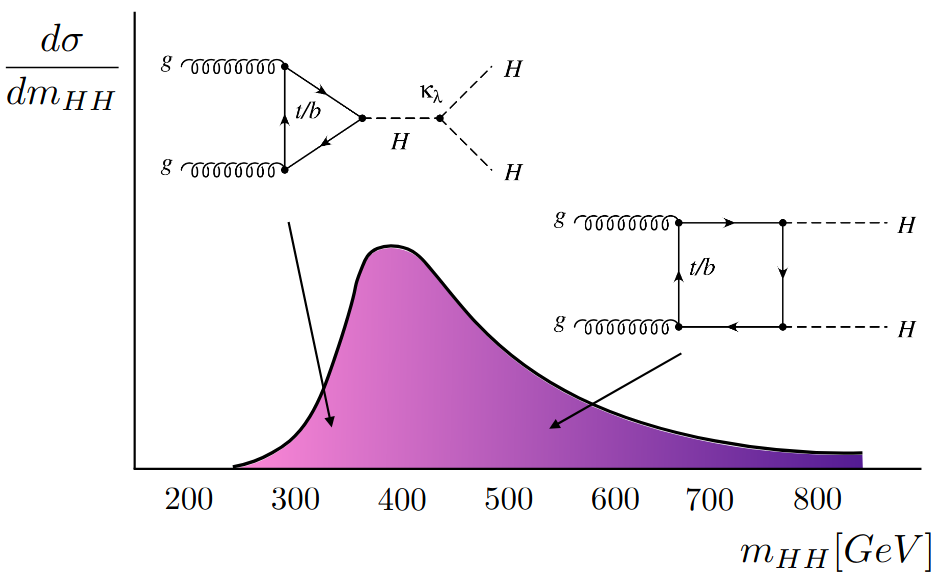
\includegraphics[width=1\textwidth]{Part3/Img/mHH_diagram2.png}
    \onslide<2->\centering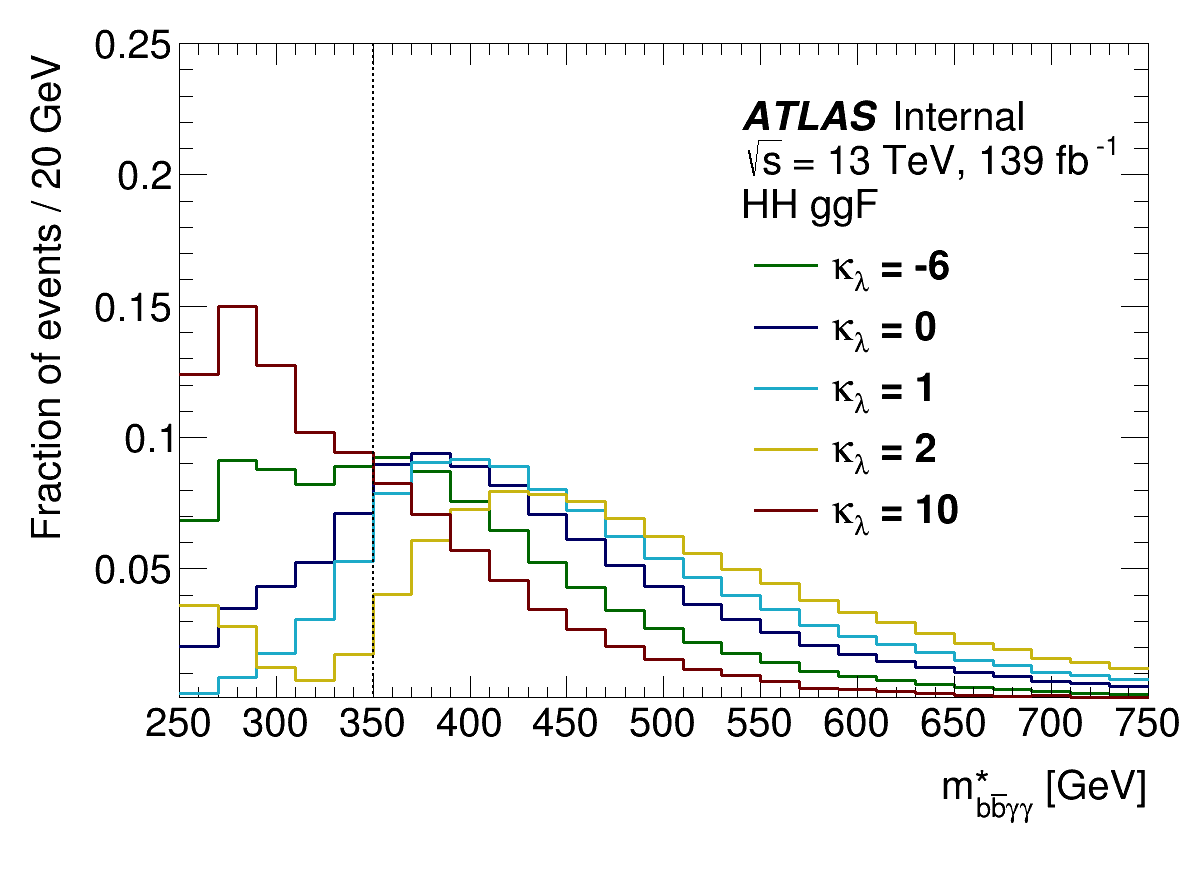
\includegraphics[width=1\textwidth]{Part3/Img/yybbstar_ggF.png}
    \end{overprint}
\end{figure}
\onslide<2->{
\begin{equation*}
    \textcolor{gray}{m_{b \bar{b}\gamma\gamma}^{*} =  m_{b \bar{b}\gamma\gamma} - m_{b \bar{b}} - m_{\gamma\gamma} + 250 \ \text{GeV}}
\end{equation*}
}
\end{columns}
\end{frame}

\begin{frame}{MVA categorization}

\begin{columns}
\column{0.6\textwidth}
\begin{itemize}
    \item Two MVA trained to discriminate signal from backgrounds:
    \begin{itemize}
        \item Low mass: \textbf{\textcolor{HHred}{SM HH ($\kappa_{\lambda} = $1)}}
        \item High mass: \textbf{\textcolor{HHturquoise_d}{BSM HH $\kappa_{\lambda} = $10}}
    \end{itemize}
    \item Similar features: object and event kinematic
    \item MVA techniques: 
    \begin{itemize}
        \item \textcolor{structurColor}{\textbf{B}oosted \textbf{D}ecision \textbf{T}rees}: signal vs ($t\bar{t}$H + ZH + continuum $\gamma\gamma$)
        \item \textbf{D}eep \textbf{N}eural \textbf{N}etwork: multi-classification
    \end{itemize}
\end{itemize}  

\column{0.4\textwidth}

\begin{figure}
    \centering
    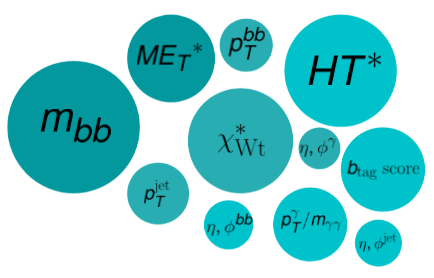
\includegraphics[width=1.\textwidth]{Part3/Img/MV_var.png}
\end{figure}
\textcolor{gray}{$^{*}$ not used in DNN} \\

%$\chi_{Wt}= \min \sqrt{\left(\frac{m_{j_{1} j_{2}}-m_{W}}{m_{W}}\right)^{2}+\left(\frac{m_{j_{1} j_{2} j_{3}}-m_{t}}{m_{t}}\right)^{2}}$

\end{columns}   
\end{frame}

\begin{frame}{Deep Neural Network selection}
\begin{columns}
\column{0.4\textwidth}
\begin{itemize}
    \item Dense network with 4 outputs
    \item $d_{HH}$ discriminates
    \begin{equation*}
        d_{HH} = \frac{\sigma_{HH}.p_{HH}}{\sum{\sigma_{bkg}.p_{bkg}}}
    \end{equation*}
    \item Good modelling of $d_{HH}$
    \item \textbf{\textcolor{HHred}{4 categories}} maximize combined expected significance 
    \item \textbf{\textcolor{HHturquoise_d}{Similar performance to the BDT}}
    \onslide<3>{
    \item baseline: \textbf{BDT}
    \item DNN for next analysis round
    }
\end{itemize}
\onslide<2-3>{
\column{0.6\textwidth}
\begin{figure}
    \centering
    \fcolorbox{gray}{HHwhite2}{
     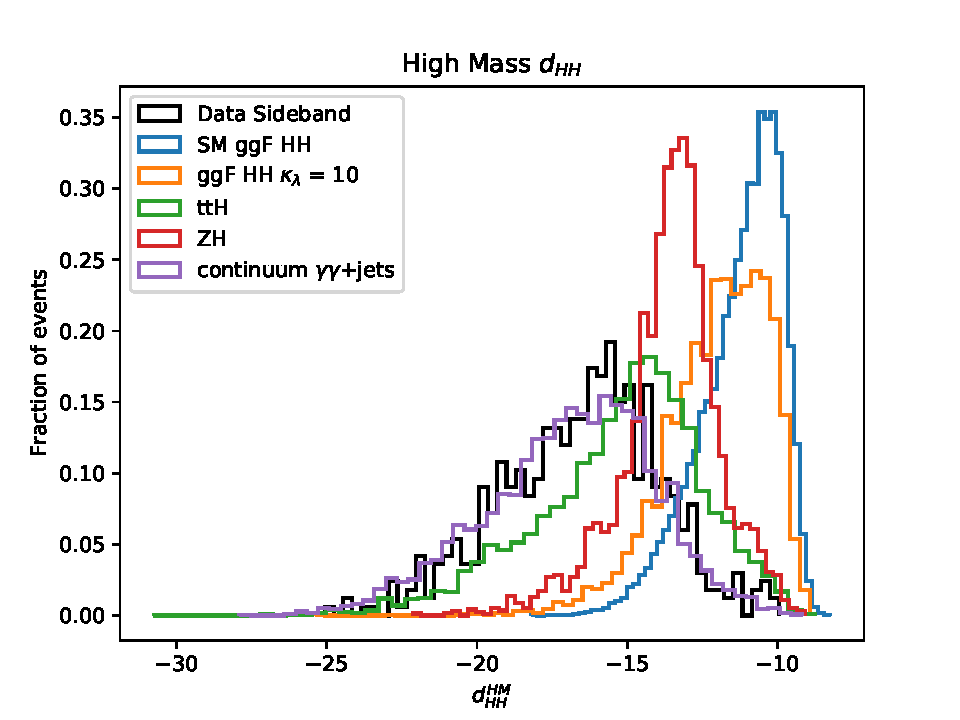
\includegraphics[width=0.65\textwidth]{Part3/Img/dHH_SM.pdf} 
     }
 %   \subfloat{ 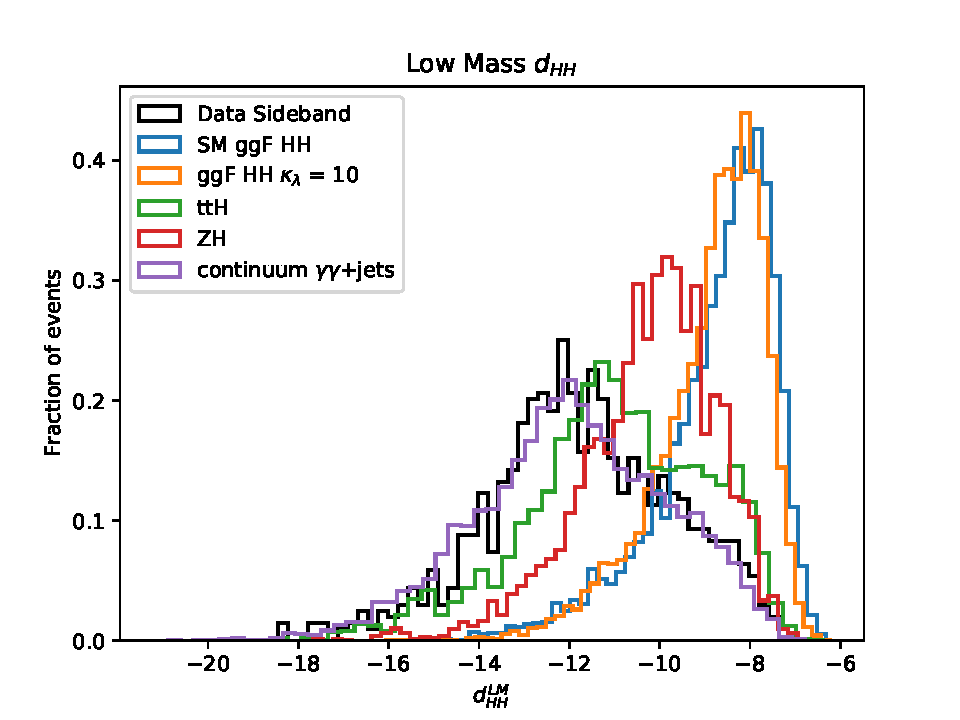
\includegraphics[width=0.55\textwidth]{Part3/Img/dHH_BSM.pdf}}
\end{figure}
}
\onslide<2-3>{
\begin{table}
    \centering
    \begin{tabular}{lcc}
    \hline\hline
        MVA & SM HH & HH $\kappa_{\lambda}$ \\
        \hline
        BDT & 0.49 & 3.59 \\
        DNN & 0.54 & 3.47 \\
        \hline\hline
    \end{tabular}
\end{table}
\begin{center}
  \textcolor{gray}{$Z = \sqrt{2[(s+b)\times\log{1+s/b}-2]}$}  
\end{center}
}
\end{columns}
\end{frame}

\begin{frame}{Signal extraction}
\begin{columns}
\column{0.5\textwidth}    
    
\begin{itemize}
    \item \textcolor{structurColor}{$m_{\gamma\gamma}$ modelling in the 4 categories}
    \item \textbf{\textcolor{red}{HH signal} (ggF + VBF)}: 
    \begin{itemize}
        \item \textbf{from Monte Carlo}
        \item \textbf{Yield parametrized as a function of $\kappa_{\lambda}$}
        \item Double-sided Crystal-Ball (DSCB)
    \end{itemize}
    \item \textbf{\textcolor{red}{Single Higgs}}: 
    \begin{itemize}
        \item \textbf{from Monte Carlo}
        \item Same PDF as the signal (injection test)
    \end{itemize}
    \item \textbf{\textcolor{blue}{Continuum $\gamma\gamma$}}:
    \begin{itemize}
        \item \textbf{fully data driven}
        \item smoothly falling analytic function 
        \item Spurious signal test: quantify model bias $\to$ systematic uncertainty
    \end{itemize}
\end{itemize}    
    
\column{0.5\textwidth}
\begin{figure}
    \centering
    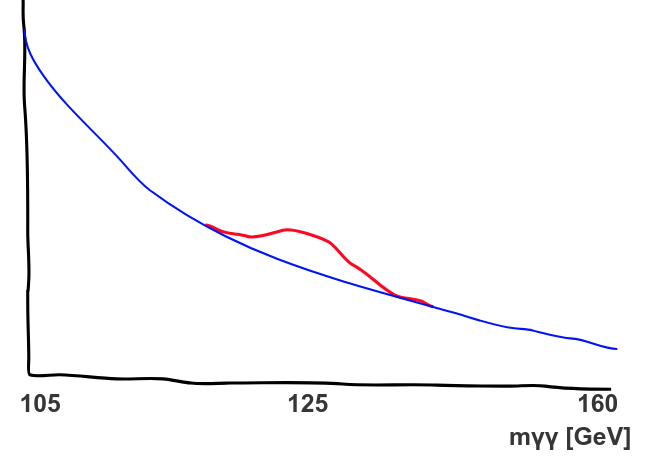
\includegraphics[width=0.8\textwidth]{Part3/Img/myysketch.png}
\end{figure}
\end{columns}
    
\end{frame}

\subsection{Higgs self-coupling constrain}

\begin{frame}{Fit results}

\begin{columns}
\column{0.5\textwidth}
\begin{itemize}
    \item Simultaneous fit 
    \item \textbf{\textcolor{HHred}{No significance SM HH signal observed}}
    \item Upper limits as a function of $\kappa_{\lambda}$ on $\sigma_{HH}$
\end{itemize}

\column{0.5\textwidth}

\begin{figure}
    \centering
    \fcolorbox{gray}{HHwhite2}{
    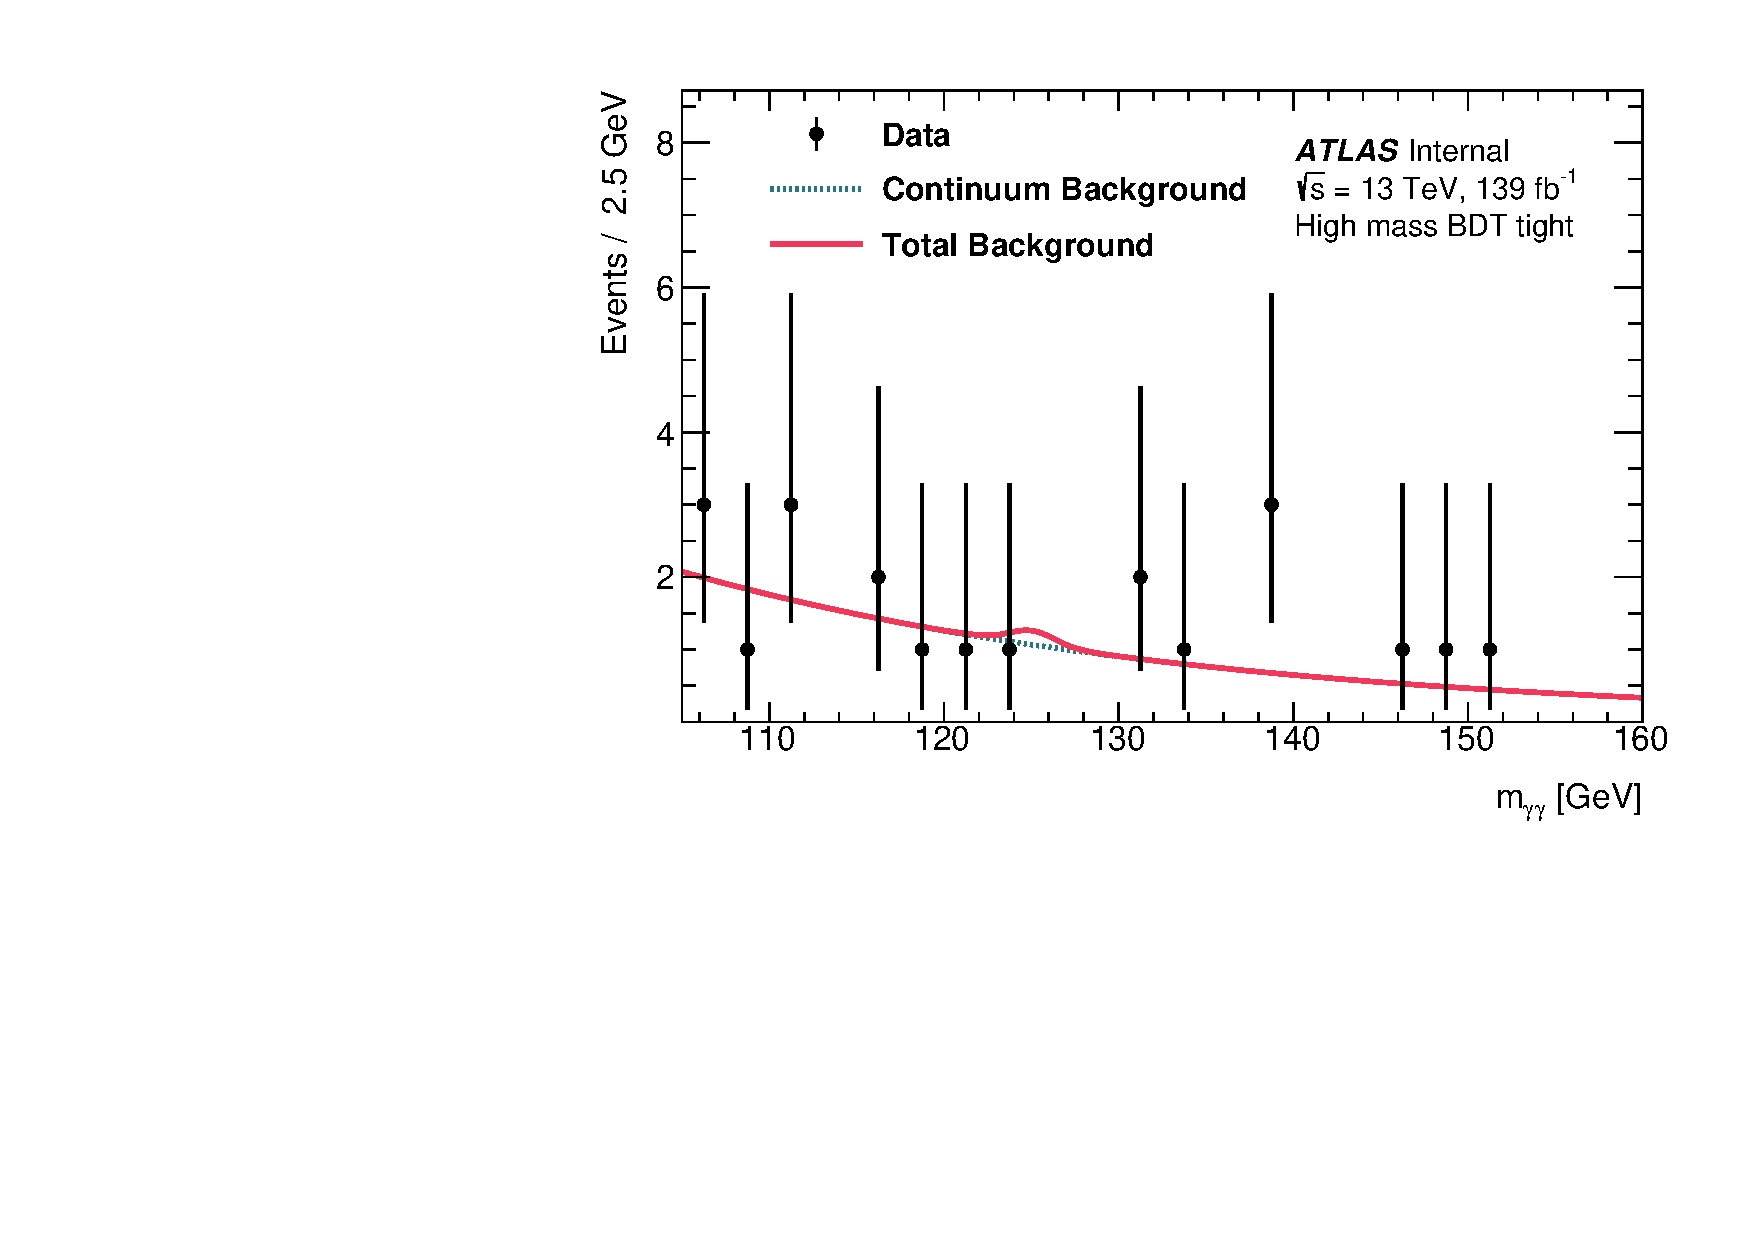
\includegraphics[width=1.\textwidth]{Part3/Img/m_yy_High_mass_Tight_BDT.pdf}
    }
\end{figure}

\begin{center}
   \textcolor{gray}{ \textbf{most sensitive category}}
\end{center}

\end{columns}    
\end{frame}


\begin{frame}{Limits and $\kappa_{\lambda}$ constrain}
\setbeamercovered{transparent}
\begin{columns}
\column{0.4\textwidth}

\begin{figure}
    \centering
    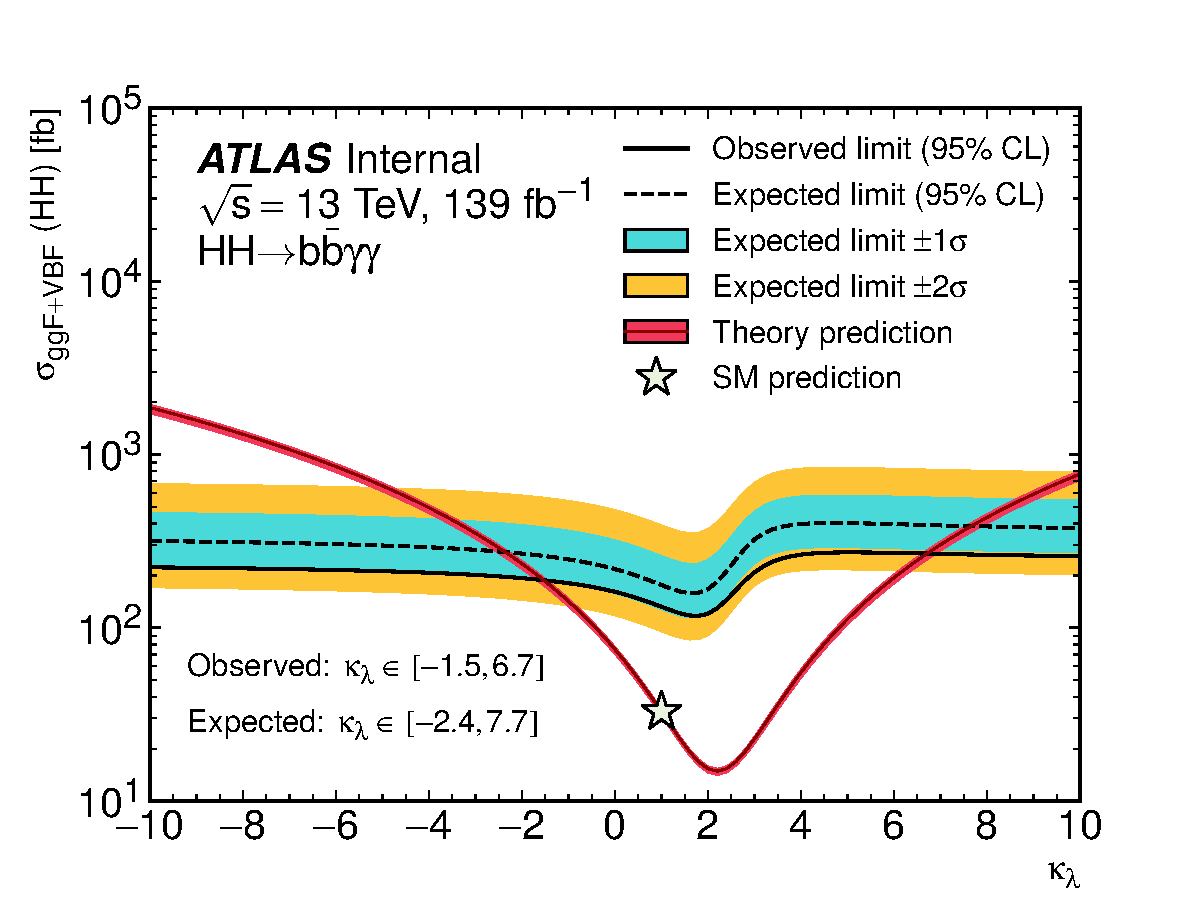
\includegraphics[width=1.1\textwidth]{Part3/Img/figures_Results_kappa_lambda_scan.pdf}
\end{figure}

\column{0.6\textwidth}

\begin{itemize}
    \item $\frac{\sigma_{HH}}{\sigma_{HH}^{SM}}$ limit: \textbf{\textcolor{HHred}{4.1}} (Exp. \textbf{5.5}) 
    \item $\kappa_{\lambda}$ constrain: \textbf{\textcolor{HHred}{[-1.5, 6.7]}} (Exp. \textbf{[-2.4, 7.7]})
    \pause
    \item \textbf{Statistically limited}
    \begin{itemize}
        \item Systematic effect $\sim$ \textbf{4\%}
        \item background modelling \& photon energy scale
    \end{itemize}
    \pause
    \item \textbf{\textcolor{cadmiumorange}{5$\times$ improvement}} w.r.t 36 fb$^{-1}$
    \begin{itemize}
        \item Increase luminosity: 2$\times$
        \item \textbf{\textcolor{HHturquoise_d}{Analysis improvement: 3$\times$}}
        \begin{itemize}
            \item$m_{HH}$ categorization and MVA strategy (\textbf{20\%})
            \item $b$-jet energy calibration (\textbf{7\%})
            \item ...
        \end{itemize}
    \end{itemize}
    \pause
    \item HH$\to b\bar{b}\tau^+\tau^-$ $\frac{\sigma_{HH}}{\sigma_{HH}^{SM}}$ limit: \textcolor{HHred}{\textbf{4.7}} (Exp. \textbf{3.9})
\end{itemize}
\end{columns}
\end{frame}

\begin{frame}{CMS HH$\to b\bar{b}\gamma\gamma$ results}

\begin{columns}
\column{0.6\textwidth}

\begin{itemize}
    \item \textbf{\textcolor{structurColor}{Different analysis strategies}}
    \begin{itemize}
        \item 14 categories
        \begin{itemize}
            \item \textbf{MVA output} and \textbf{$m_{b\bar{b}\gamma\gamma}$}
            \item \textbf{2 dedicated VBF categories} 
        \end{itemize}
        \item \textcolor{HHturquoise_d}{\textbf{2D fit}} $m_{\gamma\gamma}\times m_{b\bar{b}}$
    \end{itemize}
\end{itemize}

\begin{table}[]
    \centering
    \begin{tabular}{lcc}
    \hline\hline
    & Expected & Observed \\
    \hline 
    CMS $\frac{\sigma_{HH}}{\sigma_{HH}^{SM}}$ limit & \textbf{5.2} & 7.7 \\
    CMS $\kappa_{\lambda}$ interval & \textbf{[-2.5, 8.2]} & [-3.3, 8.5] \\
    \hline 
    ATLAS $\frac{\sigma_{HH}}{\sigma_{HH}^{SM}}$ limit & \textbf{5.5} & 4.1 \\
    ATLAS $\kappa_{\lambda}$ interval & \textcolor{HHred}{\textbf{[-2.4, 7.7]}} & [-1.5, 6.7] \\ 
    \hline\hline
    \end{tabular}
    
\end{table}

\column{0.4\textwidth}

\begin{figure}
    \centering
    \fcolorbox{HHturquoise_d}{HHwhite2}{
    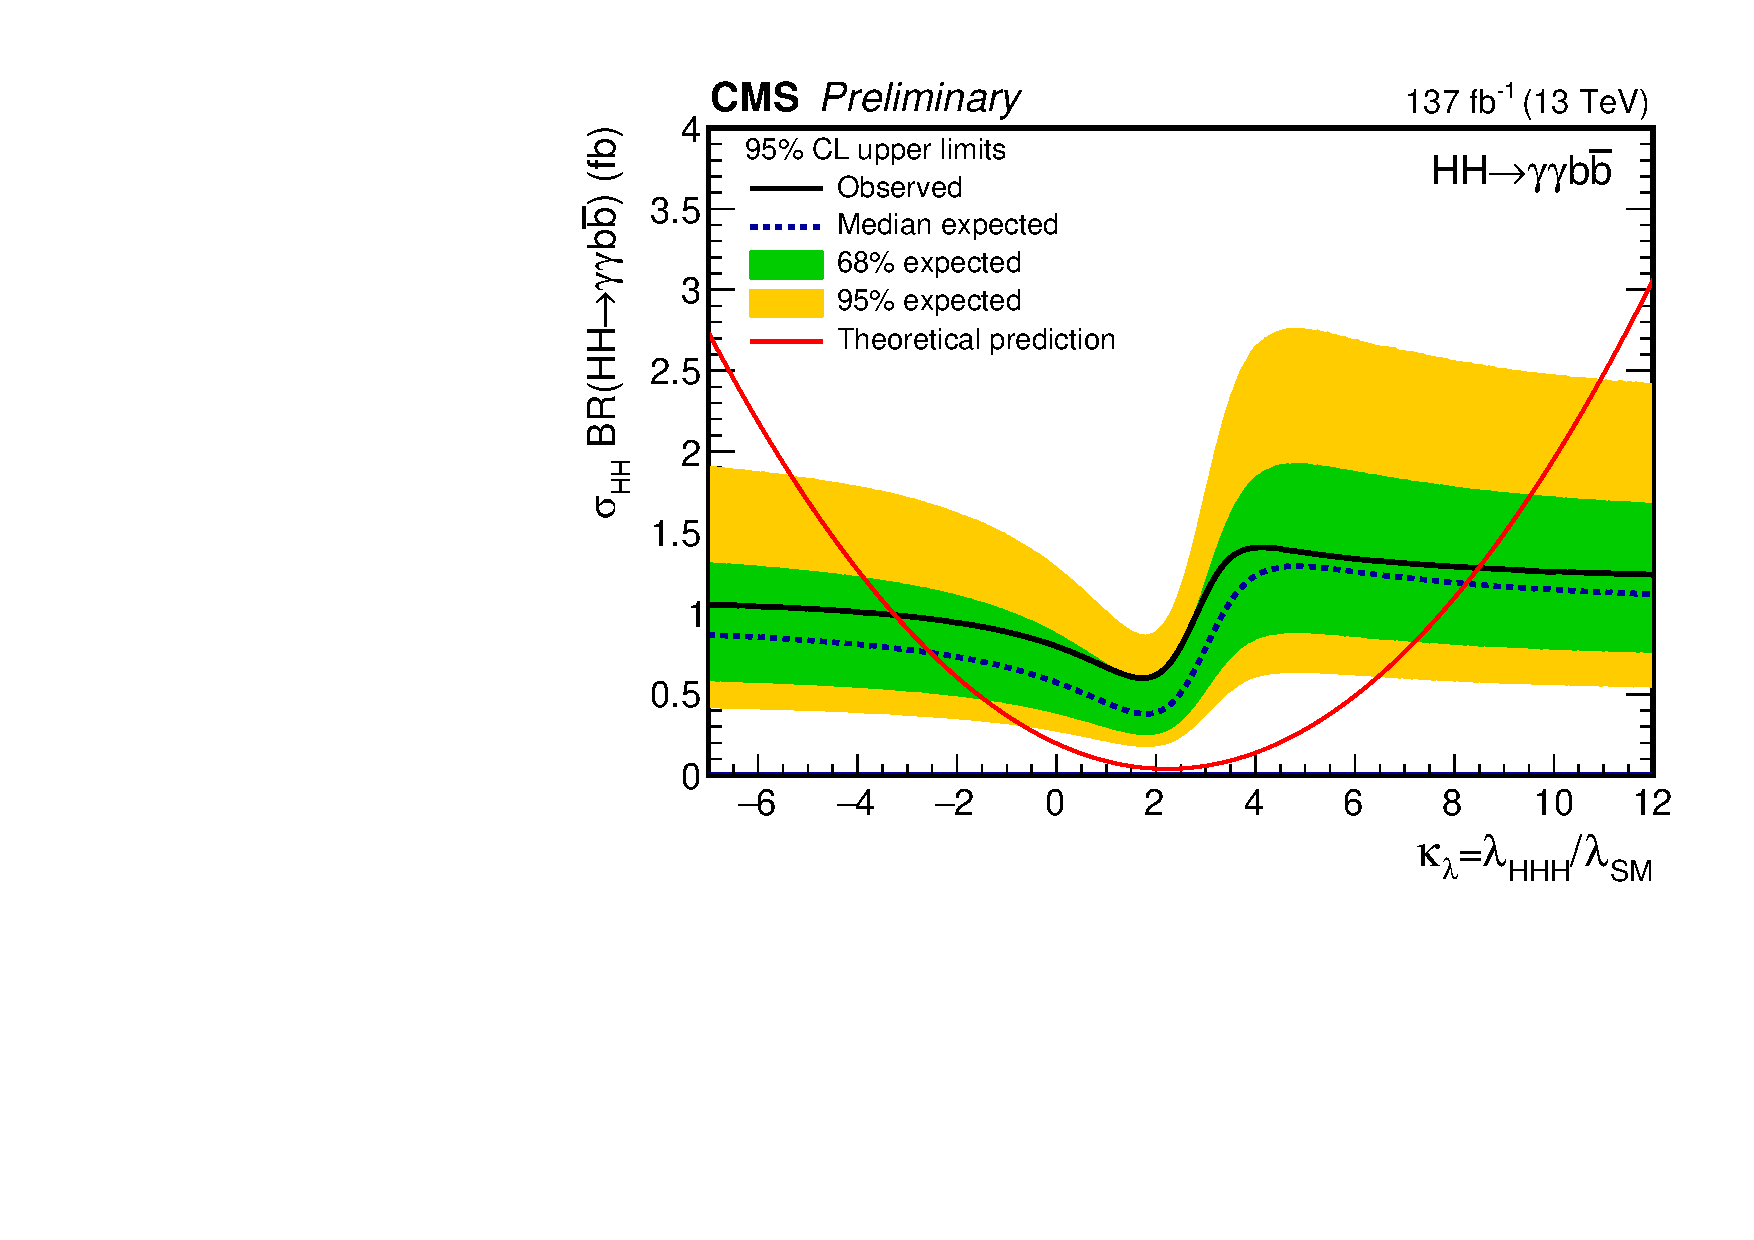
\includegraphics[width=1.\textwidth]{Part3/Img/CMS_kl_scan.pdf}
    }
\end{figure}
\end{columns}
\end{frame}

